\documentclass[12pt, a4paper, french, BCOR = 0pt, DIV = 10]{scrartcl}
\usepackage{graphicx} % Required for inserting images
\usepackage{babel}
\usepackage{amsmath}
\usepackage[utf8]{inputenc}
\usepackage[T1]{fontenc}
\usepackage{graphicx}
\usepackage{listings}
\usepackage{float}
\usepackage{subcaption}
\usepackage[toc,page]{appendix}
\graphicspath{ {./images/} }

\usepackage{bigints}

\usepackage{pxfonts}

\title{MIG Verre - Modélisation des fours}
\author{\small{Simon Lamaze - Corto Beck - Girardet Grégoire - Fraenkel Paul}}

\begin{document}
    \maketitle
    \tableofcontents
    
    \section{Introduction}
    Ce mini-projet traite de la modélisation et de l'optimisation énergétique des fours à verre.  La compréhension des phénomènes physiques qui prennt place dans un four est essentielle à l'optimisation des procédés.
    \begin{center}
        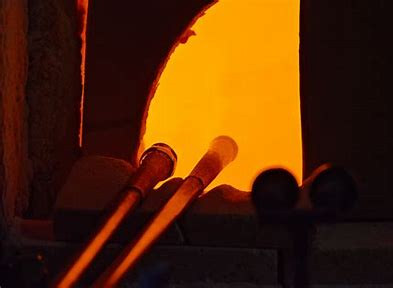
\includegraphics[width=\linewidth]{ImageIllustration.jpeg}
    \end{center}
    

    \section{Objectifs}
    \subsection{Contexte}
    Le verre est un matériau produit à des températures très élevées, de l'ordre de 1300°C. Il feut utiliser des quantités d'énergies très importantes pour porter le matériau à cette températures, et le moyen utilisé aujourd'hui est principalement l'utilisation de bruleurs au gaz (les bruleur au fioul ne sont plus utilisés pour des raisons économiques) qui ont une consommation de l'ordre du $m^{3}.s^{-1}$. Malgré des moyens mis en place pour augmenter l'éfficacité du chauffage, comme l'utilisation de préchauffage de l'air qui sert pour la combustion par un système d'alimentation alternée, cela reste particulièrement polluant. Pourtant, le verre liquide est conducteurs, ce qui signifie qu'une fois porté à suffisament haute température, il peut être chauffé par des électrodes qui créent un champ électrique dans le liquide et provoque un réchauffement par effet joule. Ce système permet de parvenir à des fours superboosté à partir de 25\% d'alimentation électrique, et à des fours hybrides à partir de 50\% d'alimentation électrique, voire à des fours complètement électriques. Cependant, des contraintes de qualité du verre empêchent l'utilisation de cette méthode pour les verres de bonne qualité, car on observe alors une augmentation de la quantité de bulles dans le verre à cause de la modification de la dynamique du four. En effet, les flux de matières sont différents selon que la chaleur provienne du haut ou du fond du four, et les boucles de convection ne permettent plus d'évacuer convenablement les bulles en faisant résider le verre dans le fours pour une durée assez longue.

    \subsection{Objectifs}
    Le but est de simuler des fours à verre alimentés principalement par source électrique, afin d'identifier les dynamiques de ces fours particuliers et permettre la conception de fours industriels fonctionnant à l'électricité qui ont donc une empreinte carbone plus faible (tant que l'électricité utlisée est verte). On s'intérresse d'abord à la compréhension des dynamiques des fours existant et connus, avant de proposer des modifications de ces outils pour utiliser plus d'électrcité. Pour ce faire, on dispose des outils du cemef et des connaissance de Franck Pigeonneau, qui maîtrise déjà les outils.
    
    \section{Principes du four à verre}
    \subsection{Introduction}
    Le but du four à verre industriel est de produire en continue un verre de la meilleur qualité possible, mais aussi de qualité uniforme, et cela en continu. Pour cela, des matières premières sont insérées dans le fours en continu, et la production de verre se fait sans arrêt pour toute la durée de fonctionnement du four (10 à 20 ans). Des boucles de convection assurent un mélange des matériaux au sein du four et un temps de résidence suffisament long pour laisser le temps aux bulles de s'évacuer. Le verre étant très visqueux (10 000 fois plus que l'eau dans le four), le matériau doit rester plusieurs jours dans le four.
    
    \begin{center}
        \begin{figure}[h]
            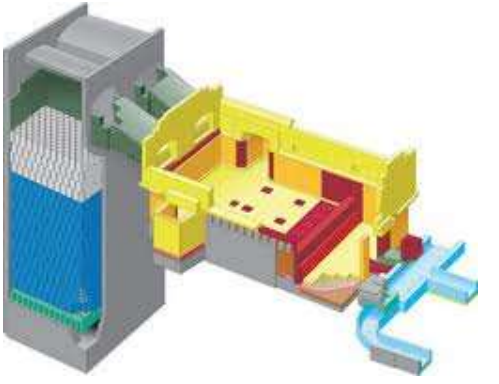
\includegraphics[width=\linewidth]{FourAVerre.png}
        \end{figure}
    \end{center}

    \subsection{Chauffage du four}
    Aujourd'hui, les fours sont alimentés principalement en gaz naturel. Pour minimiser l'énergie apportée à l'air qui sert de comburant, deux alimentation fonctionnent par alternance. Lorsque l'une sert d'entrée, l'autre sert de sortie et l'air chaud de l'intérieur passe à travers un récupérateur de chaleur. De taille très importante, cet appareil représente une part significative du coût du four mais voit son utilisation rentabilisée au bout de quelques années par les économies de gaz qu'il permet. Ainsi, lorsque l'air entre dans le four, il n'est plus à température ambiente mais déjà à plusieurs centaines de degrés.\\
    Le gaz naturel pourrais être remplacé par du dihydrogène, qui a l'avantage de pouvoir être produit par électricité. Cependant, cette méthode pose aussi des problèmes. En effet, il n'existe aujourd'hui toujours pas de réseau de distributionde dihydrogène à grande échelle ce qui signifie qu'il doit être produit sur site, principalement à partir d'hydrocarbures. De plus, les flammes de dihydrogène sont invisibles par les caméra qui sont sensibles au visible, ce qui signifie qu'elle ne sont pas compatibles avec l'équipement de surveillance actuel qui permet la gestion des flammes.

    \subsection{Géométrie du four}
    \begin{center}
        \begin{figure}[h]
            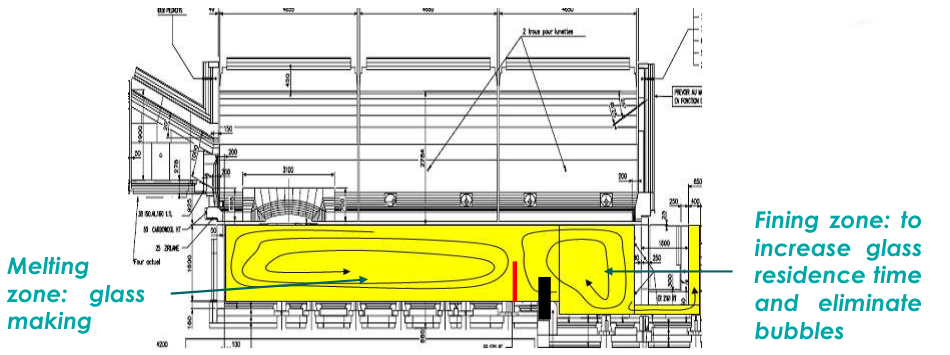
\includegraphics[width=\linewidth]{VueEnCoupe.png}
        \end{figure}
    \end{center}
    La forme du bain est étidiée pour maximiser la qualité du verre produit. Lors de son entrée, la matière est prise dans une première boucle de convection, qui lui permet de fondre et de s'homogénéiser. Cette boucle de trouve dans la plus grande zone du bain, séparée de l'autre zone par un petit muret. Celui-ci à pour but de faciliter la formation de la seconde boucle de convection, séparée de la première et qui a pour but de parfaire la préparation du verre, en éliminant les dernières bulles et en finalisant l'homogénéisation du mélange. La géométrie du bain est très importante pour la qualité finale du verre, et on se reposera sur des formes existantes pour créer notre modèle numérique afin de maximiser nos chances de trouver une forme qui fonctionne.

    \subsection{Extraction du verre}
    Une fois que le verre a fini sont parcours dans le four, il est extrait du bain par une gorge qui le mène vers des feeders. À cette étape, le verre doit atteindre sa température optimale de formage, et être maintenu assez chaud jusqu'à sont arrivée dans le moule. Pour cette raison, bien que le verre doive descendre en température, il est tout de même nécessaire de chauffer les conduite afin de garder le verre assez chaud, ce qui est une autre source d'émissions de GES.

    \section{Modèles étudiés}
    Afin de comparer les fours classiques, avec très peu de contribution électrique, et les fours hybrides, avec une puissance apportée principalement par électricité, on va modéliser deux fours de tailles identiques.

    \subsection{Four classique}
    Le premier modèle étidié est un four classique, à alimentation principalement thermique avec appoint de chauffage par courant triphasé via trois électrodes.

    \begin{center}
        \begin{figure}[H]
            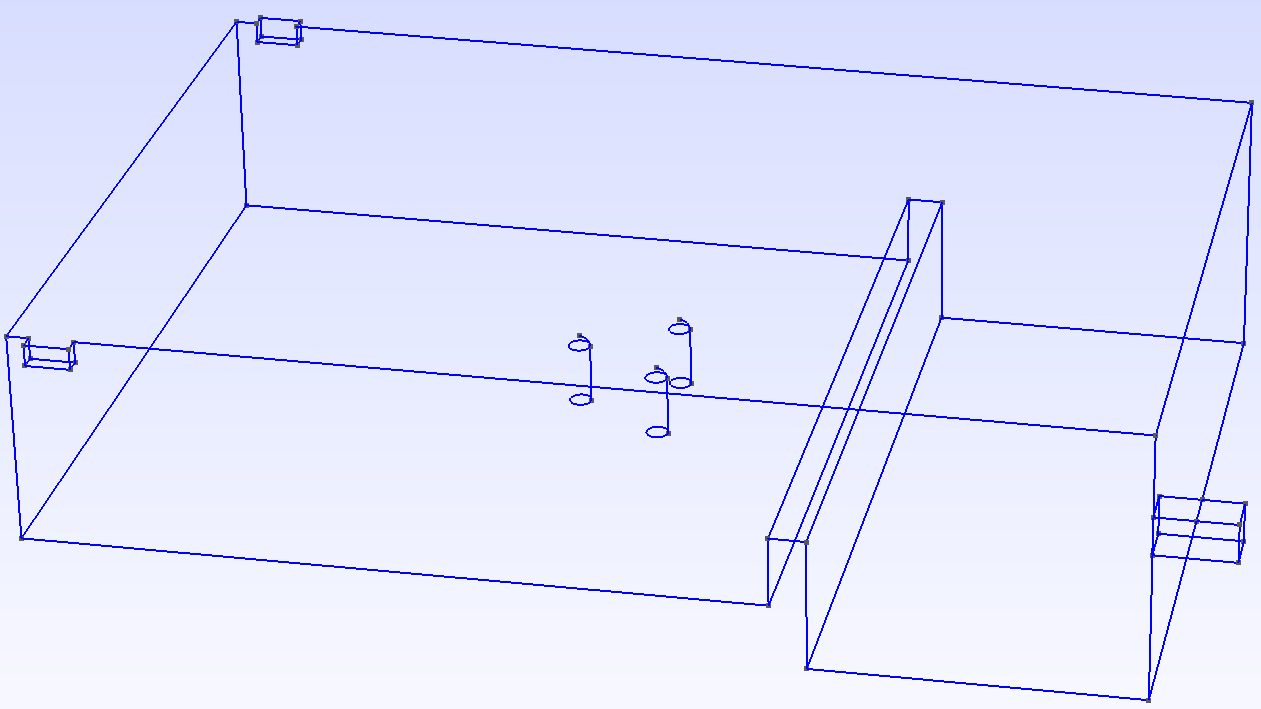
\includegraphics[width=0.7\linewidth]{FourWall.png}
        \end{figure}
    \end{center}

    On a reproduit ici la géométrie classique d'un four à verre. Les électrodes centrales permettent d'aider à la formation de la boucle de convection dans le grand bassin.
    

    \subsection{Four hybride}
    Ce modèle a pour but d'étudier le comportment du four chauffé principalemnt par les électodes. Pour limiter la densité de courant sur les électrodes et ainsi réduire la corrosion du métal, on place de nmobreuses électrodes. Elle fonctionnent par groupes de trois, dans lesquels les électrodes sont déphasées de $\frac{2\pi}{3}$ l'une par rapport à l'autre, ce qui fait qu'elles forment globalemnt trois groupes de cinq électrodes en phase, ce qui correspond à une aimentation industrielle standard en courant triphasé.

    \begin{center}
        \begin{figure}[H]
            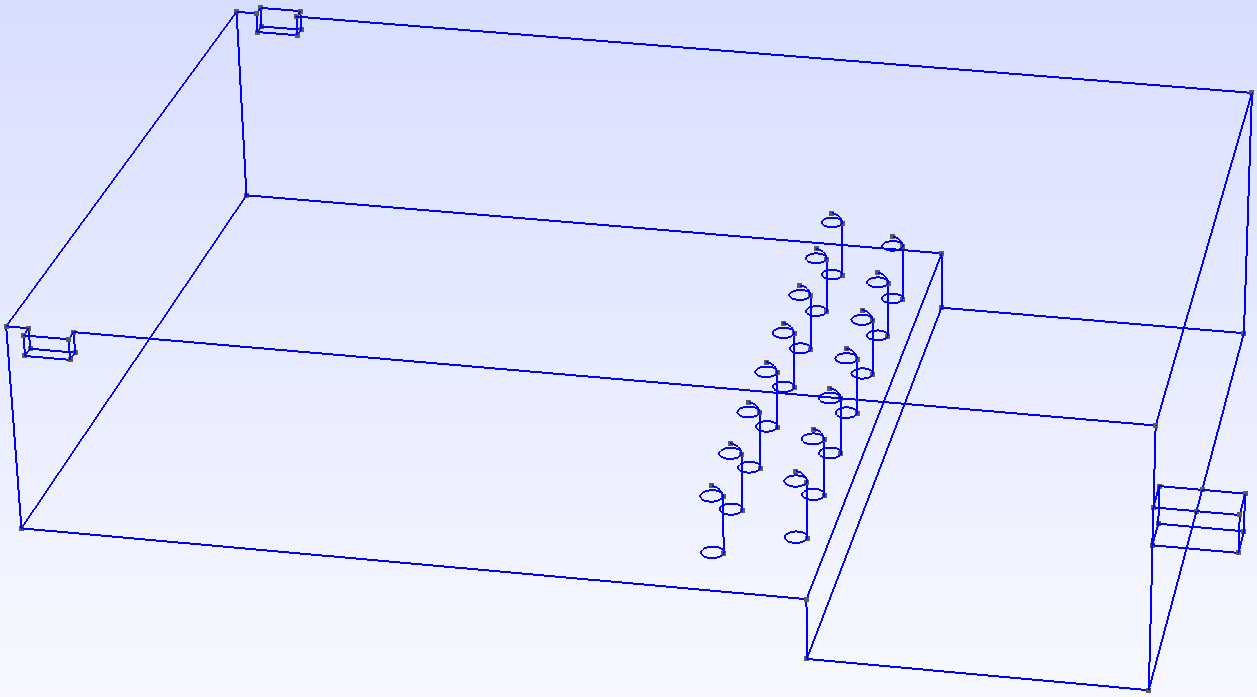
\includegraphics[width=0.7\linewidth]{Four5Elec.png}
        \end{figure}
    \end{center}




    \section{Déroulement de la simulation}
    Tâche 1 : positionnement du problème : \\
    Conditions limites, conditions initiales, mise en équations \\


    Tâche 2: prise en main des outils de calcul\\
    Maillage, cluster, post-traitement, CIMLIB, vitesse des calculs \\

    
    Tâche 3 : Calcul sur un cas à voûte chaude\\ 
    Obtenir un cas convergé, bilan énergétique \\

    
    Tâche 4 : Calcul sur un cas à voûte plus froide \\ 
    Same\\

    
    Tâche 5: Bilan du gain énergétique et des émissions carbone \\
    
    
    On  utilise le logiciel Paraview pour visualiser les résultats.
    Visualiser la propagation d'un champ pour définir le temps de résidence.
    Faire plusieurs calculs avec des tailles différentes.
    
    \section{Problèmes à résoudre}
    On va s'attcher à résoudre par méthode des éléments finis les équation qui régissent la dynamique du verre, considéré incompressible, qui sont les suivantes.
    
    \subsection{Équations du fluide}
    Les équations que nous nous appliquerons à résoudre seront les suivantes :

    \begin{figure}[H]
        \centering
        \begin{equation}
            \vec {\nabla} \cdot \vec{u} = 0
            \tag{Conservation de la masse}
            \label{eq:ConsMasse}
        \end{equation}
        \begin{equation}
            \rho_{0} \frac{D\vec{u}}{Dt} = - \vec {\nabla} P + \vec {\nabla} \cdot [ 2 \eta \vec{\mathbb{E}}] - \rho_{0} \beta (T-T_{0}) \vec{g}
            \tag{Conservation de la quantité de mouvement}
            \label{eq:ConsQteMvt}
        \end{equation}
        \begin{equation}
            \rho_{0} \left[ C_{p}+ \Delta H_{r} \frac{d\alpha}{dT} \right] \frac{DT}{Dt} = \vec {\nabla} \cdot  (\lambda_{eq} \vec{\nabla} T ) + \sigma_{e} (\vec \nabla\phi)^2
            \tag{Conservation de l'enthalpie}
            \label{eq:ConsEnth}
        \end{equation}
        \begin{equation}
            \vec{\nabla} \cdot (\sigma_{e} \vec{\nabla} \phi) = 0
            \tag{Conservation du flux électrique}
            \label{eq:ConsFluxElec}
        \end{equation}
        
    \end{figure}

    Les grandeurs en jeux sont les suivantes:
    \begin{list}{$\circ$}{}
        \item $\vec{u}$ est la vitesse du fluide
        \item $\mathbb{E}$ est le tenseur des taux de déformation: $\mathbb{E} = \frac{1}{2} (\vec{\nabla} \vec{u} + ^{\mathsf{t}}\vec{\nabla} \vec{u})$
        \item $T_{0}$ est la température de référence, à laquelle la masse volumique $\rho_{0}$ est définie
        \item $\rho$ est la masse volumique du fluide, définie par:$$\rho(T) = \rho_{0} (1 - \beta \Delta T)$$
        \item $\beta$ est le coefficient de dilatation volumique: $$\beta = -\frac{1}{\rho} \frac{\partial\rho}{\partial T}$$
        \item $\eta$ est la viscosité, modélidée par une loi de Vogel-Fulcher-Tamman: $$log~\eta = A_{\eta} + B_{\eta}\frac{1}{T - T_{\eta}}$$
        \item $\alpha$ est le taux de conversion de matière dans le bain. On considère que c'est une fonctoin d'erreur en la température pour représenter le fait que plus le bain est chaud, plus les réactions de décarbonatation qui consomme de la chaleur ont lieu
        \item $\sigma_{e}$ la conductivité électrique du milieu, donnée par: $$\sigma_{e} (T) =  A_{e} e^{\frac{-B_{e}}{T}}$$
        \item $\phi$ est le potentiel électrique. Il est complex: $\phi = \phi_{r} + i\phi_{i} $
        \item $\lambda_{eq}$ est la conductivité électrique du milieu. Comme les transfert de chaleur sous forme radiative sont très importants, on ne peut pas les négliger dans l'équation habituelle de diffusion de la chaleur: $ \rho C_{p} \frac{\partial T}{\partial t} = - \vec{\nabla} . (\lambda\vec{\nabla}T) $. Cependant, comme le milieu est semi-transparent, on peut modéliser l'ensemble des transfert en remplaçant $\lambda$ par $$\lambda_{eq} = \lambda + \frac{16n^{2} \sigma T^{3}}{3\beta_{R}} $$
    \end{list}

    On note ici $\frac{DG}{Dt}$ la dérivée particulaire de la grandeur G, qui correpond à la variation de la grandeur G le long des trajectoires des particules: $$\frac{DG}{Dt} = \lim_{\delta t \to 0} \frac{G(\vec{r}(t + \delta t), t + \delta t) - G(\vec{r}, t)}{\delta t} = \frac{\partial G}{\partial t} + \left(\vec {u} \cdot \vec {\nabla } \right) G$$

    Ces équations seront résolus autmoatiquemenr par le système de simulation, par simple déclaration du type de résolution demandé et des conditions aux limites.

        
    \subsection{État aux frontières}
    
    Les flux thermiques sont donnés par les lois de Newton et Stefan aux parois et surfaces libres. le batch est introduit à iso température. on considère les transfert thermiques de Boltzmann seulement pour la surface libre.
    On peut calculer les flux aux frontières par la loi de Newton sur les transferts conducto-convectifs.
        $$
        \phi_{wall} = h_{wall} (T - T_{\infty})
        $$
    $T_{haut, min}$ : Température minimale de voûte
    \break
    $\Delta T_{haut}$ : Différence de température maximale


    
    \subsection{Calcul de grandeurs macroscopiques}
    Les équations précédentes donnent les variations infinitésimales des différents grandeurs locales, mais on s'intéresse aussi à la manière dont elles varient globalement, notamment pour déterminer les différentes puissances en jeux dans le système.
    \paragraph{Puissance électrique}Pour déterminer la puissance fournie au fluide par le sélectrodes, on calcul en chaque point le flux la puissance, que l'on peut ensuite intégrer.\\
    En chaque volume infinitésimal $dV$, la puissance électrique dissipée est $\delta P = \sigma_{e} \vec{E}^{2} dV$, où $\vec{E} = -\vec{\nabla} \phi$. Ainsi, la puissance électrique totale est:
    $$
    P_{elec}=\iiint_{four} \sigma_{e}\left[\vec \nabla\phi\right]^2~dV  = \iiint_{four} \vec \nabla \cdot \left[\sigma_{e}\vec \nabla\phi\right]~dV
    $$
    Grâce à une intégration par partie, la loi de conservation du flux et le théorème de Green-Ostrogradski donnent:

    $$P_{elec}=\phi \int_{\partial electrode} \sigma_{e} \vec \nabla\phi \cdot \vec{n}~dS
    $$

    \paragraph{Puissances thermiques}
    Pour calculer la puissance fournie sous forme thermique par les bruleurs, on calcul l'intégrale du flux thermique à travers la surface libre dans la simulation:
    $$
        P_{bruleurs} = \iint_{surface libre} \vec{j}_{thermique} \cdot \vec{dS}
    $$

    De même, on peut calculer les pertes thermiques à travers les parois du four:
    $$
        P_{pertes} = \iint_{murs} \vec{j}_{thermique} \cdot \vec{dS}
    $$

    \subsection{Temps de résidence}
    Le temps de résidence des particules dans le four est une grandeur essentielle, qui permet de quantifier l'élimination des bulles dans le verre produit. Il existe différentes manières de le calculer.
    \paragraph{Méthode analytique}
    Cette méthode consiste à calculer la réponse du four à un dirac. Pour simplifier les calculs, on peut calculer la réponse à un échelon de particules en entrée du four, qui satisfait alors l'équation de transport $$\frac{DC}{Dt} = 0 $$On peut le faire au moyen du logiciel de simulation, a posteriori sur une solution qui a atteint le régime permanent. Pour obtenir le flux de particules qui sort du four, il suffit alors de calculer le flux moyen à travers la sortie: $$
        F = \frac{\int_{sortie} C\vec{u} \cdot \vec{dS}}{\int_{sortie} \vec{u} \cdot \vec{dS}}
    $$
    Pour obtenir la réponse à un Dirac, et donc la distribution des temps de résidence dans le four, il suffit alors de dériver par rapport au temps. On obtient alors la distribution des temps de résidence: $$
        E(t) = \frac{dF}{dt}
    $$


    % $$
    % \phi_{C} =  \oiint_S C\vec{u} \cdot \vec{n}~dS  ~~~~~~~~~~ \phi = \oiint_S \vec{u} \cdot \vec{n}~dS  ~~~~~~~~~~
    % \langle C \rangle = \frac{\phi_{C}}{\phi}
    % $$ 
    
    % La distribution des temps de résidence, à savoir la réponse à un dirac, est donnée par \[E(t)=\frac{d\langle C \rangle}{dt}\]

    \paragraph{Simulation de diffusion}
    Une autre méthode consiste à simuler la diffusion de particules dans le champ de vitesse obtenu dans une simulation qui a atteint le régime permanent. 

	
	\section{Réalisation des simulations}

    \subsection{Création du four}
    On commence par créer un maillage représentant le four à partir de ses dimensions, qui ont été déterminées préalablement. On utilise l'outil gmesh, qui génère un ensemble de points et de segments les reliants. Tous les champs, scalaires et vectoriels, seront calculés en ces points lors de la simulation. Il est donc nécessaire qu'il y en ait assez pour garantir la précision de la simulation, mais la quantité de calcul augmente avec le nombre de point. Il faut donc trouver la bonne finesse, qui peut être variable dans le maillage. On augmente la densité dans la gorge (tunnel d'évacuation du verre) et à proximité des zones de forte variation dans les champs.\\
    TODO: ajouter images du four (mesh, geométrie)\\
    Une fois le maillage crée, on converti le fichier produit en un format particulier utilisé par la bibliothèque de calcul au moyen d'un script pyhton.

    \subsection{Définition du four pour le calcul}
    Une fois que l'on dispose du maillage du four, et que l'on a décidé des paramètres de la simulation (durée, pas de temps, conditions aux limites, ...) on peut rentrer ces paramètres de façon à ce qu'ils puissent être lus par le logiciel de simulation. Pour cela, on utilise un langage de déclaration créé sur mesure pour l'outil. Tous les champs doivent être initialisés, et la façon dont ils sont calculés à chaque pas de temps est défini, au moyen de solveurs d'équations aux dérivées partielles prédéfinis.\\
    \begin{figure}
        \caption{Exemple de code pour le calcul d'une température de voute à profil gaussien}
        \label{code.1}
        \begin{lstlisting}[frame=single]
            { Operation= Xnorm = X }
            { Operation= Xnorm *= 2 }
            { Operation= Xnorm /= L }
            { Operation= Xnorm += -1 }
            { Operation= Xnorm **= 2 }
          
            { Operation= Ynorm = Y }
            { Operation= Ynorm *= 2 }
            { Operation= Ynorm /= W }
            { Operation= Ynorm += -1 }
            { Operation= Ynorm /= 3 }
            { Operation= Ynorm **= 2 }
          
            { Operation= Tvoute = Xnorm }
            { Operation= Tvoute += Ynorm }
            { Operation= Tvoute *= -1 }
            { Operation= Tvoute EXP Tvoute }
            { Operation= Tvoute *= TvouteCons }
            { Operation= Tvoute += Tbase }
        \end{lstlisting}
    \end{figure}
    Cette étape est longue et sujette à erreurs, notament à cause du nombre de champs à changer, de l'absence totale de documentation sur l'outil, et du manque de clareté des messages d'erreurs produit par l'outil lors d'un problème dans le sdéclarations.

    \subsection{Calculs de la simulation}
    Pour réaliser les calculs, on utilse le cluster du cemef: un serveur disposant de 100 noeuds de calcul, chacun disposant de deux processeurs pour un total de 64 coeurs. Une fois la simulation lancée, les taches sont réparties de façon automatique entre les coeurs pour une vitesse de calcul maximale. On peut agir sur la simulation au moyen d'un fichier lu à chaque itération qui sert d'interface homme-machine (ihm), et ainsi changer différents paramètres: température d'entrée de la matière dans le four, paramètres de l'asservissement PID, ... De plus, la simulation produit un fichier qui recense la valeur de certains paramètres à chaque itération, comme la température de sortie, les puissances électriques et thermiques fournies et les pertes thermiques à travers les parois, et des fichiers qui enregistre complètement les champs régulièrement. On peut alors surveiller l'avancement de la simulation, et agir sur les paramètres afin d'obtenit un résultat satisfaisant (les calculs étant très longs, on veut pouvoir mener à bien une simulation qui n'a pas bien commencé).

    
    \section{Simulations réalisées}
    
	
	\subsection{Première série de calculs}
	\paragraph{}
	Disposant de 4 postes de calculs , nous avons commencé par chercher à simuler un four  d'une forme ressemblant à celle d'un four industriel .


    \section{Régulation à l'aide d'un PID}
    \subsection{Asservissement en puissance électrique}
    \paragraph{Principe général et Besoin}

    Le paramètre principal à maîtriser pour un four pour un industriel est sa température de sortie. La pilotabilité de l'énergie apportée par électrodes en fait un moyen de régulation particulièrement adapté. Dans ses recherches passées, notre encadrant Franck Pigeonneau a utilisé un régulateur PID agissant sur la puissance des électrode, pour contrôler la température de sortie. La difficulté à modéliser le système formé par le bain de verre réduit la détermination des coefficients du PID à des méthodes empiriques. Nous nous proposons de réaliser une modélisation simplifiée afin de déterminer une estimation plus précise de ces coefficients.

    \paragraph{Modélisation simplifiée}
    Nous avons basé nos calculs sur le modèle de four à 5 électrodes. Puisque les boucles de convections définissent deux "domaines", il est possible de ne considérer que la seconde moitié du four menant à la sortie. Cela mène à ne considérer qu'une seule boucle de convection, qui se modélise par un retard dans le transort de la température entre les différents points du cycle.

    \paragraph{Simulation sur Simlab}
    La boucle de convection est divisée en 2 sections, reliant les 2 zones principales que sont la zone de chauffage par électrodes et la zone de sortie, où le flux de matière est divisé en deux, l'un revenant dans la boucle, et l'un sortant du système. La vitesse de déplacement de la matière dans la boucle est déterminée grâce aux simulations. La zone de chauffage produit l'échauffement de température suivant :
    
    $$\Delta T = \frac{P_{elec}}{\dot{m}\cdot C_p}$$
    
    Reste à modéliser la propagation de la chaleur aux différents points du cycle de convection. Nous pouvons comparer les temps caractéristiques de propagation de la chaleur par convection et par conduction :

    $$\tau_{Conduction} = \frac{a^2\rho C_p}{K} \approx 134 \; h$$
    $$\tau_{Convection} = \frac{d_{parcours}}{u_{moy}} \approx 133 \; s$$

    Cela invite à négliger le terme de conduction thermique, et à modéliser le transport de la température par un retard de valeur $\Delta t=d_{parcours}/u_{moy}$. Néanmoins, la conduction thermique n'étant pas totalement absente, la température n'est pas discontinue, et il convient donc de rajouter un terme pour l'étape du transport, que nous considérerons d'ordre 1 pour plus de simplicité.\\

    \paragraph{Résultats de la simulation}
    La simulation permet d'obtenir une bonne approximation de la valeur des coefficients du régulateur PID. Il apparaît à première vue que le terme le plus important est le terme proportionnel, et qu'il est possible de se passer des corrections intégrale et dérivée. On observe que le système ainsi réglé semble se comporter comme un système d'ordre 1. Theoriquement, il suffirait d'augmenter le terme proportionnel jusqu'à obtenir un dépassement pour diminuer le temps de réponse. Le système réel d'électrode étant limité en puissance, le gain $K_P$ doit lui aussi être limité.     
    Cette première simulation permet de définir les coefficients suivants :
    $$K_P=1000$$
    $$K_I=0.001$$
    $$K_D=0$$
    Le choix de ne pas prendre un terme $K_I$ nul vient du fait que nous n'avons pas pris en compte les pertes thermiques, qui engendrent un besoin en apport de puissance supérieur, compromettant la précision de la régulation limitée au terme proportionnel.

    \paragraph{Simulation du four}
    Afin d'améliorer la précision des coefficients, nous avons simulé un four avec une régulation PID utilisant les coefficients précédemment définis. On observe que la température de sortie $T_{outlet}$ sur laquelle est réalisée l'asservissement converge avec un temps de réponse à 95\% de $2.0\cdot10^4 \; s$. Ce qui est convenable. Néanmoins, comme attendu, la températude de consigne n'est pas atteinte :
    $$T_{finale}=1569.9 \;^{\circ}K ~~~~~~~~~~ T_{Cons}=1593.15 \;^{\circ}K$$
    L'anayse de l'évolution des termes du régulateur permet d'obtenir une nouvelle estimation du coefficient $K_I$

    \paragraph{Nouvelle estimation de $K_I$}
    Une vision du régulateur PID est d'utiliser le terme Intégral pour compenser toutes les pertes énergétiques en régime stationnaire, et le terme proportionnel pour réagir aux fortes variations. En effet, lorsque la température de consigne est atteinte, le terme proportionnel est alors nul. En régime stationnaire, la puissance à apporter au milieu est donnée par : 
    
    $$P_{apport}=\dot{m}C_P(T_{Cons}-T_{Inlet}) + P_{pertes} - P_{gaz}$$
     
    d'où
    $$P_{apport} \approx 25.394\;kW$$

    Grâce à la simulation Cimlib, on calcule la valeur du terme intégral $S_{Int}$ à $t=t_{95\%}$. On obtient alors :
    $$K_I = \frac{P_{apport}}{S_{Int}} \approx 0.039$$

    \subsection{Asservissement en température de voute}
    \paragraph{Principe général}
    Une autre manière de réguler la température de sortie est par le changement de la température de voute. En effet, dans notre simulation, la voute du four est considérée comme la partie chauffée au gaz, et réduire sa température tout en compensant la perte de puissance thermique avec plus de chauffage électrique est un bon moyen de réduire les émissions en $CO_{2}$ du four.

    \paragraph{Modélisation}
    Pour simplifier le système, on considère cette fois que la puissance fournie par les électrodes est constante, de valeur égale à la puissance thermique fournie en régime permanent dans la simulation avec apport principlament themrique. La température de voute est calculée selon la formule:
    $$
        T_{voute} = T_{base} + DT e^{-\vec{r}^{2}}
    $$
    avec $T_{base} = 1373,15K$ la température minimale sur la surface, qui est une température froide pour un four à verre, et DT calculé par PID. De cette manière, on obtient un profil gaussien à la surface du verre.

    \paragraph{Détermination de DT}
    On cherche à calculer DT de sorte que la température maximale à la surface du four ne dépasse pas la température maximale possible à la voute d'un four à verre, qui est d'environ 1800°C. On doit donc toujours avoir $DT < 500K$. Comme on s'attend à avoir une erreur la plus faible au début de la simulation avec $\epsilon_{0} \approx 100K$, ce qui nous donne $K_p = 2,5$ pour un temps de réponse maximal en température. On utilise cette fois $K_{i} = 10^{-5}$.

    \begin{appendices}
    \section{Commandes}
    cd /work/MINES-PARISTECH/slamaze
    sf
    nano ihm.mtc => changer le temps à 0
    cd GlassFurnace3D/
    cimlib CFD driver glassfurnace3d.mtc
    
    ls Geometrie/
    mv Geometrie/indicfrontieres.vtu /work/MINES-PARISTECH/slamaze/ => open avec PARAVIEW, vérifier les frontières
    nano ihm.mtc , modifier le temps
    sbatch job.sh
    \end{appendices}
	
\end{document}

\documentclass[12pt, a4paper, french, BCOR = 0pt, DIV = 10]{scrartcl}
\usepackage{graphicx} % Required for inserting images
\usepackage{babel}
\usepackage{amsmath}
\usepackage[utf8]{inputenc}
\usepackage[T1]{fontenc}
\usepackage{graphicx}
\usepackage{listings}
\graphicspath{ {./images/} }

\usepackage{bigints}

\usepackage{pxfonts}

\title{MIG Verre - Modélisation des fours}
\author{\small{Simon Lamaze - Corto Beck - Girardet Grégoire - Fraenkel Paul}}

\begin{document}
    
    \maketitle
    
    \section{Introduction}
    \raggedright
    Ce mini-projet traite de la modélisation et de l'optimisation énergétique des fours à verre.  La compréhension des phénomènes physiques qui prennt place dans un four est essentielle à l'optimisation des procédés. \\ [0.5 cm]
    Voici un four à fusion:
    

    \section{Objectifs}
    \subsection{Contexte}
    Le verre est un matériau produit à des températures très élevées, de l'ordre de 1300°C. Il feut utiliser des quantités d'énergies très importantes pour porter le matériau à cette températures, et le moyen utilisé aujourd'hui est principalement l'utilisation de bruleurs au gaz (les bruleur au fioul ne sont plus utilisés pour des raisons économiques) qui ont une consommation de l'ordre du $m^{3}.s^{-1}$. Pourtant, le verre liquide est conducteurs, ce qui signifie qu'une fois porté à suffisament haute température, il peut être chauffé par des électrodes qui créent un champ électrique dans le liquide et provoque un réchauffement par effet joule. Cependant, des contraintes de qualité du verre empêchent l'utilisation de cette méthode pour les verres de bonne qualité, car on observe alors une augmentation de la quantité de bulles dans le verre à cause de la modification de la dynamique du four. En effet, les flux de matières sont différents selon que la chaleur provienne du haut ou du fond du four, et les boucles de convection ne permettent plus d'évacuer convenablement les bulles.

    \subsection{Objectifs}
    Le but est de simule des verres alimentés principalement par source électrique, afin d'identifier les dynamiques de ces fours particuliers et permettre la conception de fours industriels fonctionnant à l'électricité qui ont donc une empreinte carbone plus faible (tant que l'électricité utlisée est verte). On s'intérresse d'abord à la compréhension des dynamiques des fours existant et connus, avant de proposer des modifications de ces outils pour utiliser plus d'électrcité. Pour ce faire, on dispose des outils du cemef et des connaissance de Franck Pigeonneau, qui maîtrise déjà les outils.
    
    
    
    \section{ Déroulement de la simulation}
    \raggedright
    Tâche 1 : positionnement du problème : \\
    Conditions limites, conditions initiales, mise en équations \\[0.3 cm]
    Tâche 2: prise en main des outils de calcul\\
    Maillage, cluster, post-traitement, CIMLIB, vitesse des calculs \\ [0.3 cm]
    
    Tâche 3 : Calcul sur un cas à voûte chaude\\ 
    Obtenir un cas convergé, bilan énergétique \\ [0.3 cm]
    
    Tâche 4 : Calcul sur un cas à voûte plus froide \\ 
    Same\\ [0.3 cm]
    
    Tâche 5: Bilan du gain énergétique et des émissions carbone \\ [0.5cm]
    
    
    On  utilise le logiciel Paraview pour visualiser les résultats.
    Visualiser la propagation d'un champ pour définir le temps de résidence.
    Faire plusieurs calculs avec des tailles différentes.
    
    \section{Positionnement du problème}
    - Les équations que nous nous appliquerons à résoudre seront les suivantes : \\
    \subsection{ Equations de Navier-Stokes et thermique}
    - Les équations que nous nous appliquerons à résoudre seront les suivantes : \\
    \centering
    $$
    \left\{
    \begin{array} {ll} 
        \vec {\nabla}. \vec{V} = 0  ~~~~~~~~~  conservation~de~la~masse\\
        
        \rho_{0} \frac{D\vec{V}}{Dt} = -\rho_{0} \beta (T-T_{0}) \vec{g} + \vec {\nabla} . [ 2 \eta (T) \vec{D}] - \vec {\nabla} P  ~~~~~~~~~ conservation~du~moment \\   
        
        \vec{D} = \frac{1}{2} [\vec{\nabla} \vec{V} + (\vec{\nabla} \vec{V})^t ] \\
        \rho [ C_{p}+ \Delta H_{r} \frac{d\alpha}{dT}] \frac{DT}{Dt} = \vec {\nabla} .  (\lambda_{eq}(T) \vec{\nabla} T ) + \sigma_{e}(T) (\vec \nabla\phi)^2  ~~~~~~~~~ \acute equation~de ~la~chaleur \\
        
        \vec{\nabla} . (\sigma_{e} \vec{\nabla} \phi) = 0  ~~~~~~~~~ conservation~du~flux~ \acute electrique
        
        
    \end{array}
    \right. 
    $$
    Comme les transfert de chaleur sous formes radiatives sont très importants, on ne peut pas les négliger dans l'équation habituelle de diffusion de la chaleur: $ \rho C_{p} \frac{\partial T}{\partial t} = - \vec{\nabla} . (\lambda\vec{\nabla}T) $. Cependant, comme le milieu est semi-transparent, on peut modéliser l'ensemble des transfert en remplaçant $\lambda$ par $\lambda_{eq} = \lambda + \frac{16n^{2} \sigma T^{3}}{3\beta_{R}} $.
    \\ [0.5 cm]
    
    
    \subsection{Puissance électrique}
    \raggedright
    On se place dans le cas uniphasé, en réalité, dans l'industrie le régime est triphasé, plus de calculs en annexes. \\ [0.2 cm ]
    \centering
    \[ P_{eq}=\int_\Omega \sigma_{e}(T)(\vec \nabla\phi)^2~dV  = \int_\Omega \vec \nabla[\sigma_{e}(T)\vec \nabla\phi]~dV \]\\
    \raggedright
    par intégration par partie et loi de conservation du potentiel ($ \vec{\nabla}^2 \phi = 0 $). Le théorème de Green-Ostrogradski donne: 
    
    \[ P_{eq}=\phi_{elec} \int_{\partial elec} \sigma_{e}(T)\vec \nabla\phi \cdot \vec{n}~dS\]
    \\
    Car le potentiel est constant = $\phi_{elec} $ à la rontière des électrodes. \\
    \subsection{ Expressions des différentes grandeurs et constantes}
    Le taux de conversion $\alpha$ est une sigmoïde : fonction d'erreur de Gauss\\ [0.3cm]
    
    - On modélise la dépendance de la viscosité à la température par une loi de type VFT ( Vogel-Fulcher-Tamman) \\ [0.5 cm]
    
    \centering
    $$
    \eta (T)  = 10^{A_{\eta}} e^{\frac{ln(10) B}{T-T_{\eta}}} ~~~~~~~~~ log(\eta) = A_{\eta} + \frac{B}{T-T_{\eta}}
    $$
    
    
    \raggedright
    - La dépendance de la masse volumique est : \\ [0.5 cm]
    \begin{center}
        
        
        $$
        \rho(T) = \rho_{0}  (1 - \beta \Delta T) ~~~~~~~~~ 
        \beta = -\frac{1}{\rho_{0}} \frac{d\rho}{dt}
        $$
        \\
    \end{center}
    
    
    
    - La dépendance de la conductivité électrique est : \\ [0.5 cm]
    \begin{center}
        $ 
        \sigma_{e} (T) =  A_{e} e^{\frac{-B_{e}}{T}}
        $
    \end{center}
    
    - Dérivée particulaire : ~~~~~~~( importante en méca flu )\\
    
    \begin{center}
        $ \frac{DG}{Dt}=\frac{\partial G}{\partial t} + (\vec {v} \cdot \vec {\nabla } ) G
        $ \\    
    \end{center}
    
    
    
    - Pour calculer le temps  de résidence, à savoir la réponse à un échelon C en entrée :\\ [0.5cm]
    $$
    \phi_{C} =  \oiint_S C\vec{u} \cdot \vec{n}~dS  ~~~~~~~~~~ \phi = \oiint_S \vec{u} \cdot \vec{n}~dS  ~~~~~~~~~~
    \langle C \rangle = \frac{\phi_{C}}{\phi}
    $$ 
    \\ [0.5 cm]
    La distribution des temps de résidence, à savoir la réponse à un dirac, est donnée par \[E(t)=\frac{d\langle C \rangle}{dt}\]
    
    \subsection{État aux frontières}
    
    Les flux thermiques sont donnés par les lois de Newton et Stefan aux parois et surfaces libres. le batch est introduit à iso température. on considère les transfert thermiques de Boltzmann seulement pour la surface libre.
    On peut calculer les flux aux frontières par la loi de Newton sur les transferts conducto-convectifs.\\ 
    \begin{center}
        $$
        \phi_{wall} = h_{wall} (T - T_{\infty})
        $$
    \end{center}
    
    
    
    $T_{haut, min}$ : Température minimale de voûte
    \break
    $\Delta T_{haut}$ : Différence de température maximale


	
	\section{Réalisation des simulations}

    \subsection{Création du four}
    On commence par créer un maillage représentant le four à partir de ses dimensions, qui ont été déterminées préalablement. On utilise l'outil gmesh, qui génère un ensemble de points et de segments les reliants. Tous les champs, scalaires et vectoriels, seront calculés en ces points lors de la simulation. Il est donc nécessaire qu'il y en ait assez pour garantir la précision de la simulation, mais la quantité de calcul augmente avec le nombre de point. Il faut donc trouver la bonne finesse, qui peut être variable dans le maillage. On augmente la densité dans la gorge (tunnel d'évacuation du verre) et à proximité des zones de forte variation dans les champs.\\
    TODO: ajouter images du four (mesh, geométrie)\\
    Une fois le maillage crée, on converti le fichier produit en un format particulier utilisé par la bibliothèque de calcul au moyen d'un script python.

    \subsection{Définition du four pour le calcul}
    Une fois que l'on dispose du maillage du four, et que l'on a décidé des paramètres de la simulation (durée, pas de temps, conditions aux limites, ...) on peut rentrer ces paramètres de façon à ce qu'ils puissent être lus par le logiciel de simulation. Pour cela, on utilise un langage de déclaration créé sur mesure pour l'outil. Tous les champs doivent être initialisés, et la façon dont ils sont calculés à chaque pas de temps est défini, au moyen de solveurs d'équations aux dérivées partielles prédéfinis.\\
    \begin{figure}
        \caption{Exemple de code pour le calcul d'une température de voute à profil gaussien}
        \label{code.1}
        \begin{lstlisting}[frame=single]
            { Operation= Xnorm = X }
            { Operation= Xnorm *= 2 }
            { Operation= Xnorm /= L }
            { Operation= Xnorm += -1 }
            { Operation= Xnorm **= 2 }
          
            { Operation= Ynorm = Y }
            { Operation= Ynorm *= 2 }
            { Operation= Ynorm /= W }
            { Operation= Ynorm += -1 }
            { Operation= Ynorm /= 3 }
            { Operation= Ynorm **= 2 }
          
            { Operation= Tvoute = Xnorm }
            { Operation= Tvoute += Ynorm }
            { Operation= Tvoute *= -1 }
            { Operation= Tvoute EXP Tvoute }
            { Operation= Tvoute *= TvouteCons }
            { Operation= Tvoute += Tbase }
        \end{lstlisting}
    \end{figure}
    Cette étape est longue et sujette à erreurs, notament à cause du nombre de champs à changer, de l'absence totale de documentation sur l'outil, et du manque de clareté des messages d'erreurs produit par l'outil lors d'un problème dans le sdéclarations.

    \subsection{Calculs de la simulation}
    Pour réaliser les calculs, on utilse le cluster du cemef: un serveur disposant de 100 noeuds de calcul, chacun disposant de deux processeurs pour un total de 64 coeurs. Une fois la simulation lancée, les taches sont réparties de façon automatique entre les coeurs pour une vitesse de calcul maximale. On peut agir sur la simulation au moyen d'un fichier lu à chaque itération qui sert d'interface homme-machine (ihm), et ainsi changer différents paramètres: température d'entrée de la matière dans le four, paramètres de l'asservissement PID, ... De plus, la simulation produit un fichier qui recense la valeur de certains paramètres à chaque itération, comme la température de sortie, les puissances électriques et thermiques fournies et les pertes thermiques à travers les parois, et des fichiers qui enregistre complètement les champs toutes les 100 itérations. On peut alors surveiller l'avancement de la simulation, et agir sur les paramètres afin d'obtenir un résultat satisfaisant (les calculs étant très longs, on veut pouvoir mener à bien une simulation qui n'a pas bien commencé). 
    
    \subsection{Calculs avec une nouvelle composition de verre}
    

    Le verre utilisé comprend \(65 \%\) de \(SiO_{2}\) , \(13 \% \) de CaO  et \(Na_{2}O\) à 25 \( \%\) . Pour relancer une simulation de four avec cette composition nous avons implémenté les nouveaux paramètres et calculé la température cible à iso-viscosité . La température cible est 173 degrés inférieure à celle précédente  (1420 K ) . On a ensuite cherché à comparer les rendements énergétiques et l'efficacité du four par rapport au verre précédent; cette diminution de la température cible diminue nettement l'énergie à apporter , car la température de voute, assurée par un chauffage au gaz , peut être diminuée diminuée . Diminuer la température de voute améliore donc également l'efficacité carbone du four .
    /
       
 

    \section{Régulation à l'aide d'un PID}
    \subsection{Asservissement en puissance électrique}
    \paragraph{Principe général et Besoin}

    Le paramètre principal à maîtriser pour un four pour un industriel est sa température de sortie. La pilotabilité de l'énergie apportée par électrodes en fait un moyen de régulation particulièrement adapté. Dans ses recherches passées, notre encadrant Franck Pigeonneau a utilisé un régulateur PID agissant sur la puissance des électrode, pour contrôler la température de sortie. La difficulté à modéliser le système formé par le bain de verre réduit la détermination des coefficients du PID à des méthodes empiriques. Nous nous proposons de réaliser une modélisation simplifiée afin de déterminer une estimation plus précise de ces coefficients.

    \paragraph{Modélisation simplifiée}
    Nous avons basé nos calculs sur le modèle de four à 5 électrodes. Puisque les boucles de convections définissent deux "domaines", il est possible de ne considérer que la seconde moitié du four menant à la sortie. Cela mène à ne considérer qu'une seule boucle de convection, qui se modélise par un retard dans le transort de la température entre les différents points du cycle.

    \paragraph{Simulation sur Simlab}
    La boucle de convection est divisée en 2 sections, reliant les 2 zones principales que sont la zone de chauffage par électrodes et la zone de sortie, où le flux de matière est divisé en deux, l'un revenant dans la boucle, et l'un sortant du système. La vitesse de déplacement de la matière dans la boucle est déterminée grâce aux simulations. La zone de chauffage produit l'échauffement de température suivant :
    
    $$\Delta T = \frac{P_{elec}}{\dot{m}\cdot C_p}$$
    
    Reste à modéliser la propagation de la chaleur aux différents points du cycle de convection. Nous pouvons comparer les temps caractéristiques de propagation de la chaleur par convection et par conduction :

    $$\tau_{Conduction} = \frac{a^2\rho C_p}{K} \approx 134 \; h$$
    $$\tau_{Convection} = \frac{d_{parcours}}{u_{moy}} \approx 133 \; s$$

    Cela invite à négliger le terme de conduction thermique, et à modéliser le transport de la température par un retard de valeur $\Delta t=d_{parcours}/u_{moy}$. Néanmoins, la conduction thermique n'étant pas totalement absente, la température n'est pas discontinue, et il convient donc de rajouter un terme pour l'étape du transport, que nous considérerons d'ordre 1 pour plus de simplicité.\\

    \paragraph{Résultats de la simulation}
    La simulation permet d'obtenir une bonne approximation de la valeur des coefficients du régulateur PID. Il apparaît à première vue que le terme le plus important est le terme proportionnel, et qu'il est possible de se passer des corrections intégrale et dérivée. On observe que le système ainsi réglé semble se comporter comme un système d'ordre 1. Theoriquement, il suffirait d'augmenter le terme proportionnel jusqu'à obtenir un dépassement pour diminuer le temps de réponse. Le système réel d'électrode étant limité en puissance, le gain $K_P$ doit lui aussi être limité.     
    Cette première simulation permet de définir les coefficients suivants :
    $$K_P=1000$$
    $$K_I=0.001$$
    $$K_D=0$$
    Le choix de ne pas prendre un terme $K_I$ nul vient du fait que nous n'avons pas pris en compte les pertes thermiques, qui engendrent un besoin en apport de puissance supérieur, compromettant la précision de la régulation limitée au terme proportionnel.

    \paragraph{Simulation du four}
    Afin d'améliorer la précision des coefficients, nous avons simulé un four avec une régulation PID utilisant les coefficients précédemment définis. On observe que la température de sortie $T_{outlet}$ sur laquelle est réalisée l'asservissement converge avec un temps de réponse à 95\% de $2.0\cdot10^4 \; s$. Ce qui est convenable. Néanmoins, comme attendu, la températude de consigne n'est pas atteinte :
    $$T_{finale}=1569.9 \;^{\circ}K ~~~~~~~~~~ T_{Cons}=1593.15 \;^{\circ}K$$
    L'anayse de l'évolution des termes du régulateur permet d'obtenir une nouvelle estimation du coefficient $K_I$

    \paragraph{Nouvelle estimation de $K_I$}
    Une vision du régulateur PID est d'utiliser le terme Intégral pour compenser toutes les pertes énergétiques en régime stationnaire, et le terme proportionnel pour réagir aux fortes variations. En effet, lorsque la température de consigne est atteinte, le terme proportionnel est alors nul. En régime stationnaire, la puissance à apporter au milieu est donnée par : 
    
    $$P_{apport}=\dot{m}C_P(T_{Cons}-T_{Inlet}) + P_{pertes} - P_{gaz}$$
     
    d'où
    $$P_{apport} \approx 25.394\;kW$$

    Grâce à la simulation Cimlib, on calcule la valeur du terme intégral $S_{Int}$ à $t=t_{95\%}$. On obtient alors :
    $$K_I = \frac{P_{apport}}{S_{Int}} \approx 0.039$$

    \subsection{Asservissement en température de voute}
    \paragraph{Principe général}
    Une autre manière de réguler la température de sortie est par le changement de la température de voute. En effet, dans notre simulation, la voute du four est considérée comme la partie chauffée au gaz, et réduire sa température tout en compensant la perte de puissance thermique avec plus de chauffage électrique est un bon moyen de réduire les émissions en $CO_{2}$ du four.

    \paragraph{Modélisation}
    Pour simplifier le système, on considère cette fois que la puissance fournie par les électrodes est constante, de valeur égale à la puissance thermique fournie en régime permanent dans la simulation avec apport principlament themrique. La température de voute est calculée selon la formule:
    $$
        T_{voute} = T_{base} + DT exp(Cons)
    $$
    avec $T_{base} = 1373,15K$, et 
    \section{Annexe}
    \paragraph{Liste des instructions:}
    cd /work/MINES-PARISTECH/slamaze
    sf
    nano ihm.mtc => changer le temps à 0
    cd GlassFurnace3D/
    cimlib CFD driver glassfurnace3d.mtc
    
    ls Geometrie/
    mv Geometrie/indicfrontieres.vtu /work/MINES-PARISTECH/slamaze/ => open avec PARAVIEW, vérifier les frontières
    nano ihm.mtc , modifier le temps
    sbatch job.sh
	
\end{document}
